\documentclass[12pt,a4paper]{article}
\usepackage[utf8]{inputenc}
\usepackage[T1]{fontenc}
\usepackage[croatian]{babel}
\usepackage{geometry}
\usepackage{graphicx}
\usepackage{setspace}
\usepackage{titlesec}
\usepackage{fancyhdr}
\usepackage{caption}
\usepackage{longtable}
\usepackage{array}
\usepackage{tabularx}
\usepackage{amsmath}
\usepackage{amssymb}
\usepackage{mathptmx}       % Times New Roman font
\usepackage{chngcntr}       % Za numeriranje po poglavljima

% Postavke margina
\geometry{left=2.5cm,right=2.5cm,top=2.5cm,bottom=2.5cm}

% Prored 1.5
\onehalfspacing

% ---- STILOVI NASLOVA ----
\titleformat{\section}
  {\normalfont\large\bfseries\uppercase}{\thesection.}{0.5em}{}
\titleformat{\subsection}
  {\normalfont\normalsize\bfseries}{\thesubsection.}{0.5em}{}
\titleformat{\subsubsection}
  {\normalfont\normalsize\bfseries\itshape}{\thesubsubsection.}{0.5em}{}
\titleformat{\paragraph}[hang]
  {\normalfont\normalsize\itshape}{\theparagraph.}{0.5em}{}
\titlespacing*{\paragraph}{0pt}{3.25ex plus 1ex minus .2ex}{0.5em}

\newcommand{\sectionbreak}{\clearpage}

% ---- NUMERIRANJE SLIKA I TABLICA ----
\counterwithin{figure}{section}
\counterwithin{table}{section}
\counterwithin{equation}{section}
\setcounter{secnumdepth}{4}
\setcounter{tocdepth}{4}

\addto\captionscroatian{%
  \renewcommand{\contentsname}{SADRŽAJ}%
  \renewcommand{\listfigurename}{POPIS SLIKA}%
  \renewcommand{\listtablename}{POPIS TABLICA}%
  \renewcommand{\refname}{LITERATURA}%
}

\captionsetup[figure]{font={small,bf},labelsep=period}
\captionsetup[table]{font={small,bf},labelsep=period,position=above}

\pagestyle{fancy}
\fancyhf{}
\fancyhead[L]{\small\textit{Krešimir Hartl}}
\fancyhead[R]{\small\textit{Seminar}}
\fancyfoot[L]{\small\textit{Fakultet strojarstva i brodogradnje}}
\fancyfoot[R]{\small\textit{\thepage}}
\renewcommand{\headrulewidth}{0.4pt}
\renewcommand{\footrulewidth}{0.4pt}

\begin{document}

\begin{titlepage}
    \thispagestyle{empty}
    \centering
    {\fontsize{16pt}{19pt}\selectfont SVEUČILIŠTE U ZAGREBU\\}
    {\fontsize{16pt}{19pt}\selectfont FAKULTET STROJARSTVA I BRODOGRADNJE\\}
    \vfill
    {\fontsize{28pt}{34pt}\selectfont\bfseries OSNOVE ROBOTIKE\\}
    \vspace{0.5cm}
    {\fontsize{28pt}{34pt}\selectfont\bfseries SEMINAR: ZADAĆA 3\\}
    \vfill
    \noindent
    \begin{minipage}[t]{0.48\textwidth}
        \raggedright
        {\fontsize{14pt}{17pt}\selectfont Profesor:\\}
        {\fontsize{14pt}{17pt}\selectfont Ime Prezime\\}
    \end{minipage}
    \hfill
    \begin{minipage}[t]{0.48\textwidth}
        \raggedleft
        {\fontsize{14pt}{17pt}\selectfont\bfseries Krešimir Hartl\\}
    \end{minipage}
    \vspace{1cm}
    \begin{center}
        {\fontsize{14pt}{17pt}\selectfont Zagreb, 2026.}
    \end{center}
\end{titlepage}

\pagenumbering{Roman}
\tableofcontents
\newpage
\listoffigures
\newpage

\pagenumbering{arabic}

\section{Arhitektura Sustava}
Sustav za zadatak pick-and-place s robotom UR5e koristi naprednu Domain-Driven Design (DDD) arhitekturu strukturiranu u \textit{src\_v2} paketu. Arhitektura je podijeljena na:
\begin{itemize}
    \item \textbf{Core:} Domenski modeli i pydantic konfiguracije sustava.
    \item \textbf{Adapters:} \texttt{RobotAdapter} za izravnu TCP/IP kontrolu robota (RTDE i URScript), \texttt{VisionAdapter} za upravljanje Intel RealSense kamerom, \texttt{StorageAdapter} za spremanje podataka i logova.
    \item \textbf{Usecases:} \texttt{PipelineOrchestrator} upravlja iterativnom petljom percepcije i planiranja, a \texttt{PlanningUseCase} generira kvintičke trajektorije u radnom prostoru.
\end{itemize}

\section{Kalibracija i Eye-in-Hand Konfiguracija}
Robotski sustav koristi \textit{eye-in-hand} postavu gdje je kamera montirana na sam gripper robota. 
Kako bi percepcijski rezultati sa senzora kamere bili ispravno mapirani u globalni radni prostor robota (robot base), prethodno su provedene kalibracije TCP-a (Tool Center Point) i same kamere. Matrica transformacije iz koordinatnog sustava TCP-a u koordinatni sustav kamere (\(T_{\text{cam\_from\_tcp}}\)) iznosi aproksimativno \([0.05, 0.02, -0.03]\) u translacijskom dijelu, te je pohranjena u mapi \texttt{data/camera\_calibration/}. Prilikom svake percepcijske operacije, pozicija točaka preračunava se s množenjem kalibracijskih matrica s trenutnom RTDE pozom robota.

\section{Obrada Oblaka Točaka (Point Clouds)}
Da bi se izbjegle smetnje, oblak točaka podvrgnut je obradi u \texttt{VisionAdapteru}. Svaki pojedini pogled prolazi sljedeće filtre:
\begin{enumerate}
    \item \textbf{VoxelGrid Downsampling}: Rezolucija postavljena na $5\text{ mm}$ radi smanjenja gustoće podataka za lakši ICP.
    \item \textbf{Statistical Outlier Removal}: Uklanjanje šuma (nb\_neighbors=20, std\_ratio=2.0).
    \item \textbf{Pass-through filter (Crop)}: Ograničavanje po dubini.
\end{enumerate}

U nastavku (Slika \ref{fig:pcds}) je prikazan utjecaj faza obrade za pojedine poglede, od sirovih originalnih točaka do segmentiranih i profiltriranih rezultata spremnih za stapanje.

\begin{figure}[h!]
    \centering
    \begin{tabular}{ccc}
        \includegraphics[width=0.3\textwidth]{../data/for_report/pointclouds/images/v1_original.png} &
        \includegraphics[width=0.3\textwidth]{../data/for_report/pointclouds/images/v1_filtered.png} &
        \includegraphics[width=0.3\textwidth]{../data/for_report/pointclouds/images/v1_segmented.png} \\
        \small (a) P1: Original & \small (b) P1: Filtrirano & \small (c) P1: Segmentirano \\
        \includegraphics[width=0.3\textwidth]{../data/for_report/pointclouds/images/v2_original.png} &
        \includegraphics[width=0.3\textwidth]{../data/for_report/pointclouds/images/v2_filtered.png} &
        \includegraphics[width=0.3\textwidth]{../data/for_report/pointclouds/images/v2_segmented.png} \\
        \small (d) P2: Original & \small (e) P2: Filtrirano & \small (f) P2: Segmentirano \\
    \end{tabular}
    \caption{Prikaz 2D projekcija Point Cloud podataka kroz faze obrade za Pogled 1 i Pogled 2.}
    \label{fig:pcds}
\end{figure}

Nakon pojedinačne obrade, scene se stapaju u jedan globalni model (\textit{Stitching}). Metoda \textbf{Colored ICP} uzima u obzir kako geometrijsku zakrivljenost tako i boju točaka. To sprječava problem lažnog "klizanja" algoritma kod homogenih površina stola i garantira oštro, stopljeno preklapanje ciljanih elemenata (Slika \ref{fig:final_pcd}). Konačan oblak isproduciran je i spremljen kao \texttt{04\_final\_merged\_point\_cloud.pcd}.

\begin{figure}[h!]
    \centering
    \includegraphics[width=0.7\textwidth]{../data/for_report/pointclouds/images/final_merged.png}
    \caption{Završno stapanje scene primjenom Colored ICP metode}
    \label{fig:final_pcd}
\end{figure}

\section{Detekcija Objekata i Lokalizacija}
Sustav detektira objekte pomoću YOLO algoritma na RGB slikama svake od tri perspektive. Ako model pronađe masku voća (npr. banana, jabuka, itd.), odgovarajući pikseli izdvajaju se na poravnatoj (aligned) Depth slici. 

Segmentirani dio dubinske slike prosljeđuje se \texttt{PointCloudProcessor}-u te stvara lokalni 3D model objekta. Centroid (točka hvatišta) izračunava se traženjem težišta prosječnih koordinata filtriranih točaka. Primjer dobivenih centroida objekata (banana) transformiranih u globalnu bazu jesu: $[-0.622, 0.144, 0.090]$ i $[-0.685, 0.089, 0.078]$. Ti podaci trajno su spremljeni u \texttt{objects\_with\_robot\_coords.json}.

\section{Generiranje i Analiza Trajektorije}
Prilikom operacije podizanja objekta, sustav kreira sigurnu kvintičku interpolaciju (polinomi 5. stupnja) koja osigurava neprekinutu i glatku brzinu te ubrzanje iz položaja HOME do položaja APPROACH i PICK (koji se nalazi malo iznad centroida detektiranog predmeta).

Generirane rute uzimaju u obzir maksimalne dopuštene brzine (\(v_{\text{max}}\)) i ubrzanja (\(a_{\text{max}}\)) definiranih robotom. Pet glavnih poza (Home, Approach, Pick, Approach Place, Place) povezane su interpolacijama radnog prostora u vremenu. 

Na slici 1 prikazan je graf kinematike trajektorije, na kojem se očituju glatke promjene na x osi bez diskontinuiteta u brzini ($\dot{x}$) i ubrzanju ($\ddot{x}$).

\begin{figure}[h!]
    \centering
    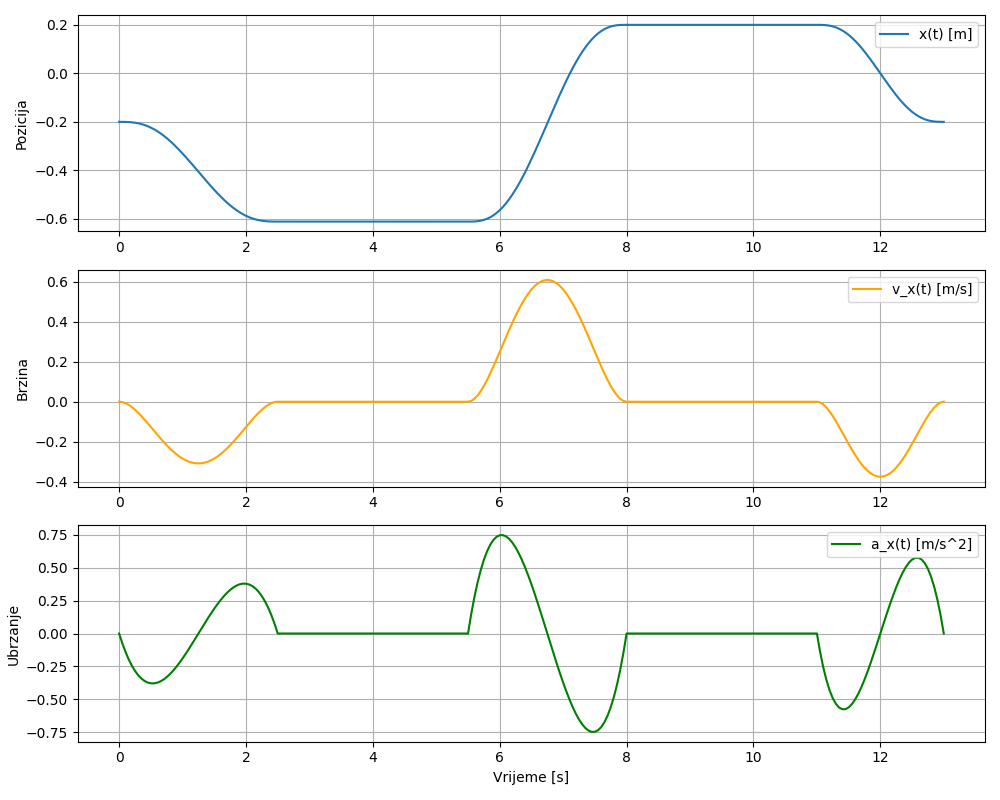
\includegraphics[width=0.8\textwidth]{../data/for_report/planning/last_trajectory_kinematics.png}
    \caption{Zapis kinematičkog planiranja trajektorije: Pozicija, Brzina, Ubrzanje}
    \label{fig:kinematics}
\end{figure}

\section{Zaključak i Reprodukcija}
Projekt u cijelosti zadovoljava zahtjeve kontinuiranog prepoznavanja voća te glatkog izvršavanja pick-and-place ciklusa na UR5e robotu. Optimizirani ICP prag smanjio je \textit{ghosting} na modelima, a DDD arhitektura omogućava brze iteracije.
Za reprodukciju sustava potrebno je instalirati okruženje pomoću \texttt{requirements.txt} te pokrenuti CLI alat na jedan od sljedećih načina:
\begin{verbatim}
# Setup okruženja
python -m venv .venv
.venv\Scripts\activate
pip install -r requirements.txt

# Offline demonstracija
python src_v2/main.py demo-offline

# Puni live sustav
python src_v2/main.py run
\end{verbatim}

\end{document}
